\subsection{Pixel Tracker Calibrations}

The CMS SiPixel detector is integral to the High-Level Trigger (HLT) decision-making process. This part of the report delves into the calibration prospects of the SiPixel detector, emphasizing unused records, FED cabling, gain and quality calibrations, CPE conditions, and alignment practices. Future prospects and recommendations for improving calibration workflows under the NGT framework are also discussed.
Out of the 326 conditions in the HLT GT, 13 are related to the Silicon Pixel Tracker, of which 12 are relevant to Run 3 data-taking. From these, the following 8 are considered core and critical for data-taking:

\begin{table}[h!]
    \centering
    \begin{adjustbox}{max width=\textwidth}
    \begin{tabular}{p{3.5cm}|p{4cm}|p{2.5cm}|p{2cm}|p{4.5cm}}
        \textbf{Name} & \textbf{Record} & \textbf{Workflow} & \textbf{Frequency of Updates} & \textbf{Description} \\ \hline
    \end{tabular}
    \end{adjustbox}
    \caption{Fundamental Silicon Strip Tracker Calibrations, ordered in terms of frequency of updates.}
    \label{tab:PixelCalibrations_critical}
\end{table}

\subsubsection{Unused Records in SiPixel Calibration}
Several records remain unused at HLT but hold relevance for other operational aspects:
\begin{itemize}
    \item \texttt{SiPixelDetVOffRcd}: Lists detector IDs with HV or LV off. Payload is ideal or empty.
    \item \texttt{SiPixelGainCalibrationOfflineRcd}: Stores gain and pedestal values for offline analysis.
    \item \texttt{SiPixelLorentzAngleRcd ("from alignment")}: Contains Lorentz Angle offsets, outdated since 2017.
    \item \texttt{SiPixelTemplateDBObjectRcd ("0T")}: Used during 0T templated tracking for PixelRecHits.
\end{itemize}

\subsubsection{FED Cabling and Calibration Maps}
The \texttt{SiPixelFedCablingMapRcd} records cabling maps connecting FEDs to readout channels. While not a direct calibration, this record plays a vital role in detector topology and reconstruction. This was last updated in 2017 with the transition to the Pixel Phase-1 detector.

\subsubsection{Bad components}
Description: This payload contains the DetIDs and ROCs associated with those DetIDs that are considered "dead." Used by tracking.\\
Record Name: \texttt{SiPixelQualityRcd} 

\subsubsection{Pixel Lorentz Angle}
Description: The 'no label' payload contains the value of LorentzAngle / Tesla for the Barrel Pixel and Forward Pixel separately (due to different HV constants, geometry, etc.).\\
Record Name: \texttt{SiPixelLorentzAngleRcd} 
Labels = none, \texttt{fromAlignment} or \texttt{forWidth} - given when included in a global tag.
\begin{itemize}
\item \texttt{fromAlignment} : the LA offset generated by alignment (alternative to LA correction from templates).
\item \texttt{forWidth}: the LA for charge width estimate in the generic CPE (alternative to the same LA as for offset). 
\end{itemize}

\subsubsection{Pixel Templates}
Description: used in the templated tracking algorithm for Pixel RecHits.
Record Name:  \texttt{SiPixelTemplateDBObjectRcd} 

\subsubsection{Generic Errors}

Description: used in the generic CPE (cluster position estimation) algorithm as errors. Improves irradiation bias corrections (IBC) for data.
Record Name:  \texttt{SiPixelGenErrorDBObjectRcd}

\subsubsection{Pixel Alignment}
Records used: 
\begin{itemize}
\item \texttt{TrackerAlignmentErrorRcd} (for alignment), 
\item \texttt{TrackerSurfaceDeformationRcd} (for surface deformation)  \item \texttt{GlobalPositonRcd} (defining the relative position of the subdetectors) 
\end{itemize}

Tracker alignment is tightly coupled with CPE conditions to mitigate Lorentz Angle miscalibrations. High-granularity offline PCL helps optimize biases but is prone to weak modes.
HLT reconstruction uses the Pixel CPE Fast algorithm (a variant of the generic algorithm), while offline operations rely on Pixel Template reconstruction. Discrepancies between these algorithms necessitate customized alignment procedures.

\begin{figure}[htbp]
   \centering
	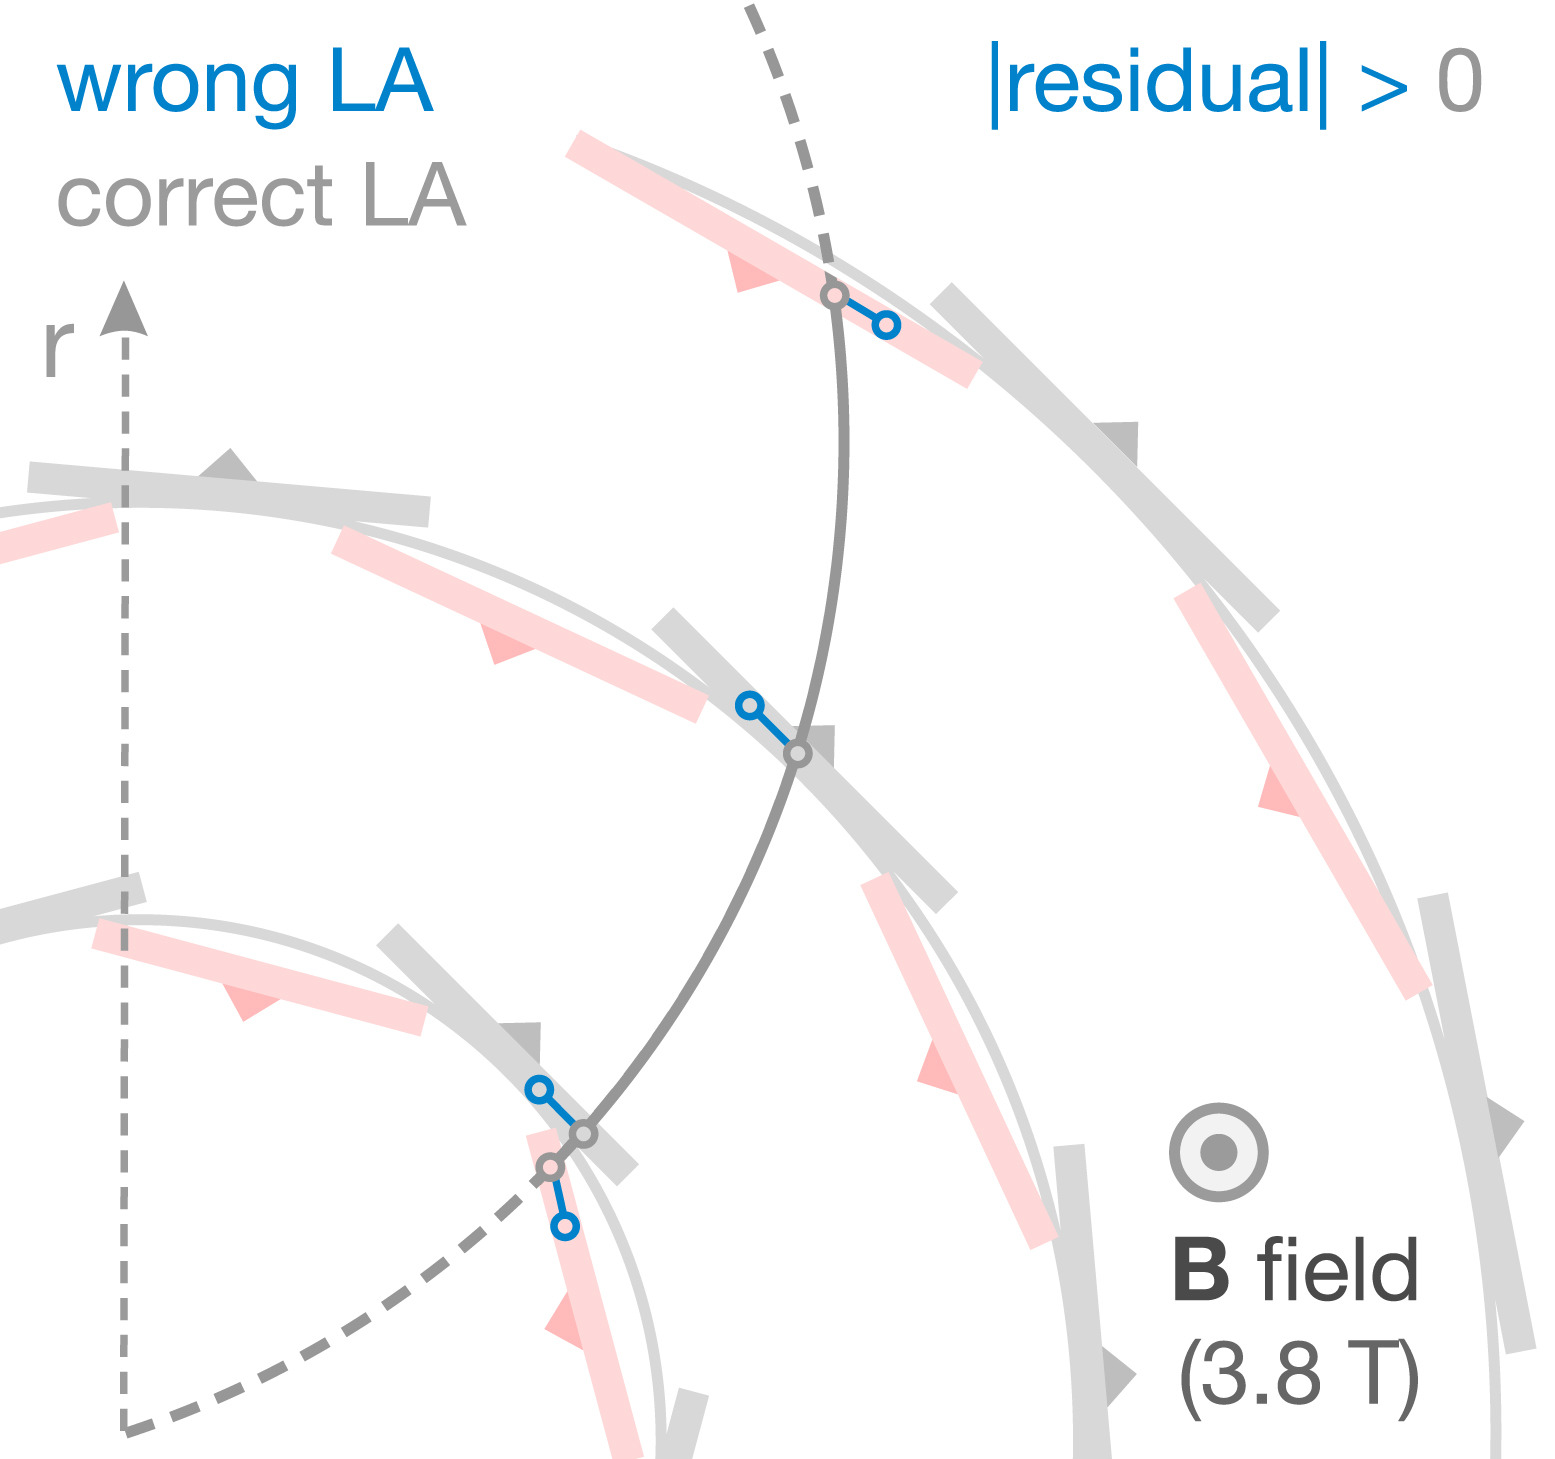
\includegraphics[width=0.5\textwidth]{figures/pixel_alignment_sketch.png}
   \caption{Sketch showing the transverse view of the Phase-0 barrel pixel subdetector, made of successive layers of silicon modules. The alternating orientation of the modules within each layer is indicated by the triangles. The blue (grey) circles represent the reconstructed hit positions using incorrect (correct) Lorentz angles in the presence of a magnetic field . The grey curve corresponds to a track built from the hits that were reconstructed with the correct Lorentz angles. Hits reconstructed with incorrect Lorentz angles are displaced in a direction defined by the orientation of the module, increasing the residual distance between the hits and the track. \cite{CMS:2022ali}}
   \label{fig:pixelAlignment}
\end{figure}

\subsubsection*{Future Prospects and Integration in NGT Demonstrator Workflow}
\begin{itemize}
    \item \textbf{Bad Components Masking}:
    \begin{itemize}
        \item Already implemented in PCL workflows and requires minimal statistics for updates.
        \item Demonstrated to improve track building in inside-out muon reconstruction.
    \end{itemize}
    \item \textbf{Pixel Alignment}:
    \begin{itemize}
        \item Enhancing alignment directly impacts B-tagging and physics trigger performance.
        \item Requires tailored workflows to address weak modes effectively.
    \end{itemize}
\end{itemize}

\subsubsection*{Recommendations}
\begin{itemize}
    \item Prioritize the inclusion of bad components masking in the NGT demonstrator workflow due to its operational simplicity and demonstrated impact.
    \item Develop alignment calibration workflows that directly integrate HLT tracks to ensure compatibility.
    \item Evaluate the feasibility of frequent updates for gains and CPE conditions to maintain precision.
\end{itemize}